
\OPGAVE
{
\section{Generaliseerbaarheidstheorie - Voorbeeld 1}

Het practicum ontwikkelingspsychologie II bestaat uit een schriftelijk verslag met 10 vragen dat elke student dient in te vullen. Deze worden door twee beoordelaars ge\"{e}valueerd waarbij elke beoordelaar alle 10 de vragen scoort.\\
Na toepassing van een variantie-analyse wordt de volgende schatting van de variantiecomponenten bekomen:

\begin{center}
\renewcommand{\arraystretch}{1.2}
\begin{tabular}{|c|c|c|c|c|c|c|c|} \hline
 & $ \hat{\sigma}^2_{s} $ & $ \hat{\sigma}^2_{v} $& $ \hat{\sigma}^2_{b} $ & $ \hat{\sigma}^2_{sv} $ & $ \hat{\sigma}^2_{sb} $ & $ \hat{\sigma}^2_{vb} $ & $ \hat{\sigma}^2_{svb,e} $ \\ \hline
Waarde  & $ 0.397 $ & $ 0.109 $ & $ 0.010 $ & $ 0.314 $ & $ 0.067 $ & $ 0.006 $ & $ 0.224 $ \\
\% Var & $ 35 $ & $ 10 $ & $ 1 $ & $ 28 $ & $ 6 $ & $ 1 $ & $ 20 $ \\ \hline
\end{tabular}
\end{center}


\normalsize
De gegevens uit de tabel kunnen gebruikt worden om volgende vragen te beantwoorden.

\begin{enumerate}
\item JUIST of FOUT: ``Idealiter is $ \hat{\sigma}^2_{s} $ substantieel groter dan $ \hat{\sigma}^2_{v}$"?
\item Stel, de verantwoordelijke lesgever zou graag in volgende jaren de werklast voor de beoordelaars opsplitsen (situatie $b$).
Beoordelaar 1 zou dan enkel vraag 1-5 verbeteren, terwijl beoordelaar 2 vraag 6-10 zou verbeteren.
Hoe ziet ons model eruit, gebruik makende van de symbolen $s$, $v$ en $b$?
\item Bereken de generaliseerbaarheidsco\"{e}ffici\"{e}nt (G) voor deze nieuwe situatie ($b$).

\item Stel, de verantwoordelijke lesgever vraagt zich af of wel alle 10 de vragen noodzakelijk zijn. Bepaal met behulp van een $D$-studie de hoeveelheid vragen die minimaal nodig is (gebruik makend van 2 beoordelaars) en toch een meetnauwkeurigheid van 0.85 te behouden.

\end{enumerate}
}

\OPLOSSING
{
\textbf{Oplossingen}
\begin{enumerate}
\item JUIST
\item $s \times v(b)$
\begin{center}
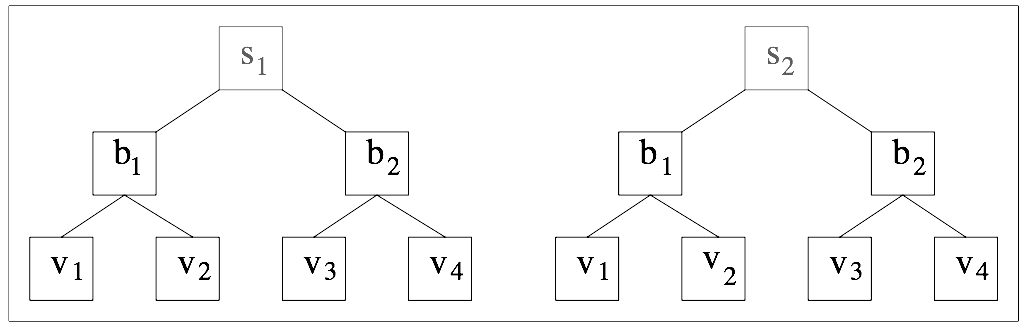
\includegraphics[scale=0.3]{sxvb.png}
\end{center}
\newpage
\item De G-co\"{e}ffici\"{e}nt wordt als volgt berekend:\\
	% G-coefficient
	\begin{align}
		G &=\dfrac{\sigma^2_{Obj~v.~met.}}{\sigma^2_{Obj~v.~met.}+ \sigma^2_{rel.~meting}} \label{eq.G1}
	\end{align}
	Merk op dat we hier te maken hebben met de volgende niet te onderscheiden variantiecomponenten:~ \\
	$ \bm{\hat{\sigma}^2_{v}} $~en~$\bm{\hat{\sigma}^2_{vb} }$.\\
	We kunnen dus enkel gebruik maken van de volgende gegevens: \\
	\begin{tabular}{|c|c|c|c|c|c|c|c|} \hline
	 & $ \hat{\sigma}^2_{s}$ & $ \hat{\sigma}^2_{b} $& $ \hat{\sigma}^2_{v,vb} $ & $ \hat{\sigma}^2_{sb}$ & $\hat{\sigma}^2_{sv} $ & $ \hat{\sigma}^2_{vb} $& $ \hat{\sigma}^2_{sv, svb, e} $ \\ \hline
	$\sigma$  			& $ 0.397 $ 			& $ 0.010 $ 			& $0.109+0.006  $ 			& $ 0.067 $				 & $. $	& $ . $& $ 0.314 + 0.224  $ \\
	$n_.$				& .						& 2					& 20				 		& 2			  		 & $. $	& $ . $&  20 \\ \hline
	$\sigma / n$ 		& .						& 0.005				& 0.00575				 		& 0.0335			  	 & $. $	& $ . $&  0.269 \\ \hline
	\end{tabular} \\

  We berekenen hiervoor eerst $\sigma^2_{rel.~meting}$
  \begin{align*}
    \sigma^2_{rel.~meting} 	&=  \dfrac{\hat{\sigma}^2_{sb}}{n_b} + \dfrac{\hat{\sigma}^2_{sv,svb,e}}{n_v*n_b} \\
                &=  \dfrac{{0.067}}{2} + \dfrac{{0.314 + 0.224}}{10*2}\\
                &= 0.0335 + 0.0269 \\
                &= 0.0604
  \end{align*}
  Bijgevolg kan $G$ opgesteld worden door $\sigma^2_{rel.~meting}$ en $\hat{\sigma}^2_{s}$ in te vullen in vergelijking \ref{eq.G1}:
  \begin{align*}
    G 	&=\dfrac{0.397}{0.397 + 0.0604}\\
      &=0.87
  \end{align*}
\item We berekenen voor de vector \textbf{v} = \{9,8,7,6,5,4,3,2,1\}, aantal vragen die aangeboden worden, telkens de G-co\"{e}ffici\"{e}nt. Deze is gelijk aan:

\begin{center}
\renewcommand{\arraystretch}{1.2}
\hspace*{-3 cm}
\begin{tabular}{|l|c|c|c|c|c|c|c|c|c|} \hline
 \textbf{v} & $ 9 $ & $ 8 $& $ 7 $ & $ 6 $ & $ 5 $ & $ 4 $ & $ 3 $ & $ 2 $ & $ 1 $ \\ \hline
G  & 0.$8623145$ & $0.855373$ & $0.8466108$ & $0.8352034$ & $0.8197398$ & $0.7975892$ & $0.7632169$ & $0.7026549$ & $0.5675482$ \\ \hline
\end{tabular}
\end{center}
We besluiten dus dat 8 vragen voldoende zijn om een meetnauwkeurigheid van 0.85 te behalen.
\end{enumerate}
}


\OPGAVE
{
\section{Generaliseerbaarheidstheorie - Voorbeeld 2}

Een verkorte vorm van de TAT (Thematic Apperception Test), bestaande uit 10 kaarten, wordt afgenomen bij 50
jongvolwassen delinquenten ($d$).
De TAT is zo opgesteld dat de juveniele delinquent bij elk van de 10 kaarten ($k$) een verhaal moet vertellen dat aansluit bij de tekening op de kaart.
De tien verhalen werden op video opgenomen en later beoordeeld.
3 klinische psychologen ($p$) beoordeelden elk de graad van \emph{rejection of authority} op een schaal van 0 tot 100.
De finale score op de TAT is het gemiddelde van de 30 metingen per subject. \footnote{
Naar Hoofdstuk 8 oef 3.a uit Crocker and Algina (2008). \emph{Introduction to Classical and Modern Test Theory}.}

\begin{center}
\renewcommand{\arraystretch}{1.2}
\begin{tabular}{|c|c|c|c|c|c|c|c|} \hline
 & $ \hat{\sigma}^2_{d} $ & $ \hat{\sigma}^2_{k} $& $ \hat{\sigma}^2_{p} $ & $ \hat{\sigma}^2_{dk} $ & $ \hat{\sigma}^2_{dp} $ & $ \hat{\sigma}^2_{kp} $ & $ \hat{\sigma}^2_{dkp,e} $ \\ \hline
Waarde  & $ 167.64 $ & $ 3.211 $ & $615.8 $ & $ 1.3 $ & $ 84.7 $ & $ 1.3 $ & $ 1.2 $ \\
\% Var & 0.1923& 0.004& 0.704& 0.001& 0.097& 0.001& 0.001 \\ \hline
\end{tabular}
\end{center}

\normalsize
De gegevens uit de tabel kunnen gebruikt worden om volgende vragen te beantwoorden.

\begin{enumerate}
	\item Schrijf deze opstelling uit.
	\item JUIST of FOUT: ``In deze opstelling kunnen er meer variantie-componenten worden onderscheiden dan wanneer elke $p$ een beperkte (unieke) set van vragen toebedeeld krijgt. Bvb. $p_1$ beoordeelt kaarten 1-4, $p_2$ kaarten 5-8 en tot slot $p_3$ kaarten 9 en 10"?
	\item Bereken de generaliseerbaarheidsco\"{e}ffici\"{e}nt (G) voor dit design.
	\item \emph{tip: schrijf bij deze vraag telkens eerst het opzet uit}\\
	Welke variantie-componenten kunnen niet meer van elkaar onderscheiden worden indien ...
\begin{itemize}
	\item ... $p_1$ vragen 1-4 beoordeelt, $p_2$ vragen 5-8 en $p_3$ vragen 9 en 10?
	\item ... door tijdsgebrek 25 subjecten kaarten 1-3 aangeboden kregen en 25 andere subjecten kaarten 4-6; bovendien beoordeelt $p_1$ kaarten 1 en 4, $p_2$ kaarten 2 en 5 en $p_3$ kaarten 3 en 6.
\end{itemize}
\item Bereken voor het eerste scenario uit (d) de $G$-co\"{e}ffici\"{e}nt en voor het tweede scenario de index of dependability $\phi$. Waar ligt het verschil tussen beide maten?
\end{enumerate}
}

\OPLOSSING
{
\textbf{Oplossingen}
\begin{enumerate}
\item JUIST.
\item $d \times k \times p$
\begin{figure}[H]
\begin{adjustwidth}{}{-0in}
\begin{center}
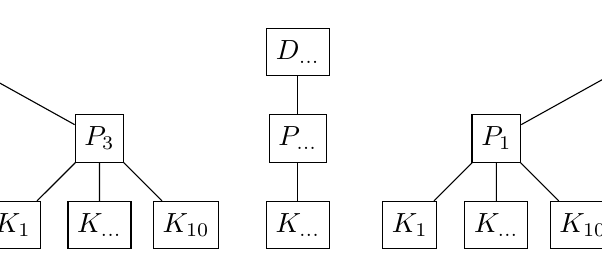
\begin{tikzpicture}[
scale=0.55,
level distance=20mm,
level 1/.style={sibling distance=36mm},
level 2/.style={sibling distance=20mm},
level 3/.style={sibling distance=12mm},
level 4/.style={sibling distance=12mm}
]

\usetikzlibrary{shapes}
\tikzstyle{c} = [draw, shape=rectangle, minimum size = 6mm]
\tikzstyle{r} = [draw, shape=rectangle,minimum width=10mm]
\tikzstyle{tr} = [draw,isosceles triangle, shape border rotate=90, anchor=north]

\hspace*{-4.5 cm}

\node[c] {$D_{1}$}
child{node[c]{$P_{1}$}
	child{node[c]{$K_{1}$}}
	child{node[c]{$K_{\ldots}$}}
	child{node[c]{$K_{10}$}}
	}
child{node[c]{$P_{2}$}
	child{node[c]{$K_{\ldots}$}}
	}
child{node[c]{$P_{3}$}
	child{node[c]{$K_{1}$}}
	child{node[c]{$K_{\ldots}$}}
	child{node[c]{$K_{10}$}}
	}
;\hspace*{4.5 cm}
\node[c] {$D_{...}$}
child{node[c]{$P_{...}$}
	child{node[c]{$K_{\ldots}$}}
	}
;\hspace*{4.5 cm}
\node[c] {$D_{50}$}
child{node[c]{$P_{1}$}
	child{node[c]{$K_{1}$}}
	child{node[c]{$K_{\ldots}$}}
	child{node[c]{$K_{10}$}}
	}
child{node[c]{$P_{2}$}
	child{node[c]{$K_{\ldots}$}}
	}
child{node[c]{$P_{3}$}
	child{node[c]{$K_{1}$}}
	child{node[c]{$K_{\ldots}$}}
	child{node[c]{$K_{10}$}}
	}
;

\end{tikzpicture}
\caption{D = delinquent, P = psycholoog en K = kaart. ``$\ldots$" = alle overige waarden. }\label{f.gen}
\end{center}
\end{adjustwidth}
\end{figure}

\item
\begin{itemize}
	\item Het opzet wordt hier: $d \times k\left(p\right)$ bijgevolg kunnen de variantiecomponenten $\sigma_p$ en $\sigma_{kp}$ niet onderscheiden worden van elkaar (wordt $\sigma_{pk,p}$) en ook $\sigma_{dp}$ kan niet van de residuele variantie-term worden onderscheiden (wordt $\sigma_{dp, dpk,e}$). Dit zijn de te onderscheiden componenten:\\ Merk hierbij op dat het object van meting $d$ is. \\
	\begin{tabular}{|c|c|c|c|c|c|c|c|} \hline
	 & $ \hat{\sigma}^2_{d}$ & $ \hat{\sigma}^2_{k} $& $ \hat{\sigma}^2_{p,kp} $ & $ \hat{\sigma}^2_{dk}$ & $\hat{\sigma}^2_{kp} $ & $ \hat{\sigma}^2_{dp} $& $ \hat{\sigma}^2_{dp, dkp, e} $ \\ \hline
	$\sigma$  			& $ 167.64 $ 			& $ 3.211 $ 			& $615.8+1.3  $ 			& $ 1.3 $				 & $. $	& $ . $& $ 1.2 + 84.7  $ \\
	$n_.$				& .						& 10					& 30				 		& 10			  		 & $. $	& $ . $&  30 \\ \hline
	$\sigma / n$ 		& .						& 0.3211				& 20.57				 		& 0.13			  	 & $. $	& $ . $&  2.8633 \\ \hline
	\end{tabular} \\
	\begin{figure}[H]
\begin{adjustwidth}{}{-0in}
\begin{center}
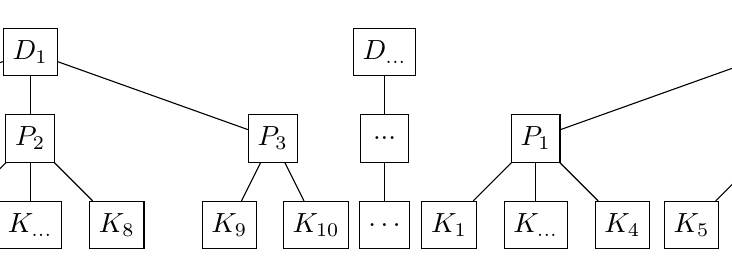
\begin{tikzpicture}[
scale=0.55,
level distance=20mm,
level 1/.style={sibling distance=56mm},
level 2/.style={sibling distance=20mm},
level 3/.style={sibling distance=12mm},
level 4/.style={sibling distance=12mm}
]

\usetikzlibrary{shapes}
\tikzstyle{c} = [draw, shape=rectangle, minimum size = 6mm]
\tikzstyle{r} = [draw, shape=rectangle,minimum width=10mm]
\tikzstyle{tr} = [draw,isosceles triangle, shape border rotate=90, anchor=north]

\hspace*{-4.5 cm}

\node[c] {$D_{1}$}
child{node[c]{$P_{1}$}
	child{node[c]{$K_{1}$}}
	child{node[c]{$K_{\ldots}$}}
	child{node[c]{$K_{4}$}}
	}
child{node[c]{$P_{2}$}
	child{node[c]{$K_{5}$}}
	child{node[c]{$K_{\ldots}$}}
	child{node[c]{$K_{8}$}}
	}
child{node[c]{$P_{3}$}
	child{node[c]{$K_{9}$}}
	child{node[c]{$K_{10}$}}
	}
;\hspace*{4.5 cm}
\node[c] {$D_{...}$}
child{node[c]{{...}}
	child{node[c]{$\ldots$}}
	}
;\hspace*{5 cm}
\node[c] {$D_{50}$}
child{node[c]{$P_{1}$}
	child{node[c]{$K_{1}$}}
	child{node[c]{$K_{\ldots}$}}
	child{node[c]{$K_{4}$}}
	}
child{node[c]{$P_{2}$}
	child{node[c]{$K_{5}$}}
	child{node[c]{$K_{\ldots}$}}
	child{node[c]{$K_{8}$}}
	}
child{node[c]{$P_{3}$}
	child{node[c]{$K_{9}$}}
	child{node[c]{$K_{10}$}}
	};
\end{tikzpicture}
\caption{D = delinquent, P = psycholoog en K = kaart. ``$\ldots$" = alle overige waarden analoog aan $D_1$ en $D_{50}$. }\label{f.gen2A}
\end{center}
\end{adjustwidth}
\end{figure}

	
	\item Het opzet wordt hier: $k\left(p\times d\right)$ bijgevolg kunnen de variantiecomponenten $\sigma_k$ en $\sigma_{kp}$, $\sigma_{kd}$ niet onderscheiden worden van  van de residuele variantie-term worden onderscheiden (wordt $\sigma_{k, kp, kd, dpk, e}$).\\Dit zijn de te onderscheiden componenten:\\ Merk hierbij opnieuw op dat het object van meting $d$ is. \\
	\begin{tabular}{|c|c|c|c|c|c|c|c|} \hline
	 & $ \hat{\sigma}^2_{d} $ & $ \hat{\sigma}^2_{k} $& $ \hat{\sigma}^2_{p} $ & $ \hat{\sigma}^2_{dk} $ & $ \hat{\sigma}^2_{dp} $ & $ \hat{\sigma}^2_{kp} $ &
	 $\sigma_{k, kp, dk, dpk, e}$ \\ \hline
	$\sigma$  			& $ 167.64 $ 			& $. $ 			& $615.8 $ 	  & $.$				 & $84.7 $	& $ . $& $ 1.2 + 84.7 +  3.211 +1.3$ \\
	$n_.$ 				& $.$ 	& $.$			& 3			  & $.$		  		 & $3*10$	& $ . $&  3 *10 \\ \hline
	$\sigma / n_.$     & .				& $. $			& $205.2333$  & $.$			  	 & $2.8233$	& $ . $&  0.0603 \\ \hline
	\end{tabular} \\
	\begin{figure}[H]
\begin{adjustwidth}{}{-0in}
\begin{center}
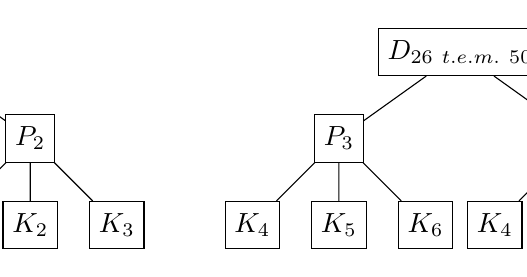
\begin{tikzpicture}[
scale=0.55,
level distance=20mm,
level 1/.style={sibling distance=56mm},
level 2/.style={sibling distance=20mm},
level 3/.style={sibling distance=12mm},
level 4/.style={sibling distance=12mm}
]

\usetikzlibrary{shapes}
\tikzstyle{c} = [draw, shape=rectangle, minimum size = 6mm]
\tikzstyle{r} = [draw, shape=rectangle,minimum width=10mm]
\tikzstyle{tr} = [draw,isosceles triangle, shape border rotate=90, anchor=north]

\hspace*{-4.5 cm}

\node[c] {$D_{1~t.e.m.~25}$}
child{node[c]{$P_{1}$}
	child{node[c]{$K_{1}$}}
	child{node[c]{$K_{2}$}}
	child{node[c]{$K_{3}$}}
	}
child{node[c]{$P_{2}$}
	child{node[c]{$K_{1}$}}
	child{node[c]{$K_{2}$}}
	child{node[c]{$K_{3}$}}
	}
;\hspace*{7 cm}
\node[c] {$D_{26~t.e.m.~50}$}
child{node[c]{$P_{3}$}
	child{node[c]{$K_{4}$}}
	child{node[c]{$K_{5}$}}
	child{node[c]{$K_{6}$}}
	}
child{node[c]{$P_{4}$}
	child{node[c]{$K_{4}$}}
	child{node[c]{$K_{5}$}}
	child{node[c]{$K_{6}$}}
	}
;
\end{tikzpicture}
\caption{D = delinquent, P = psycholoog en K = kaart. }\label{f.gen2B}
\end{center}
\end{adjustwidth}
\end{figure}

\end{itemize}
%v <- c(167.64,3.211,615.8,1.3,84.7,1.3,1.2)
%np =3
%nk =10

\item Respectievelijk de $G$ en $\phi$ co\"effici\"ent:
\begin{itemize}
	% G-coefficient
	\item
	\begin{align}
		G &=\dfrac{\sigma^2_{Obj~v.~met.}}{\sigma^2_{Obj~v.~met.}+ \sigma^2_{rel.~meting}} \label{eq.G}
	\end{align}
	Houd voorts rekening met volgende niet te onderscheiden variantiecomponenten:~ \\
	$ \bm{\hat{\sigma}^2_{p,kp}} $~en~$\bm{\hat{\sigma}^2_{dp, dkp, e} }$.\\
	We berekenen hiervoor eerst $\sigma^2_{rel.~meting}$
	\begin{align*}
		\sigma^2_{rel.~meting} 	&=  \dfrac{\hat{\sigma}^2_{dk}}{n_k} + \dfrac{\hat{\sigma}^2_{dp,dpk,e}}{n_p*n_k} \\
								&=  \dfrac{{1.3}}{10} + \dfrac{{1.2 + 84.7}}{3*10}\\
								&= 0.13 + 2.8633 &=2.9933
	\end{align*}
	Bijgevolg kan $G$ opgesteld worden door $\sigma^2_{rel.~meting}$ en $\hat{\sigma}^2_{d}$ in te vullen in vergelijking \ref{eq.G}:
	\begin{align*}
		G 	&=\dfrac{167.64}{167.64+ 2.9933}\\
			&=\dfrac{167.64}{170.6333}&=0.9825
	\end{align*}

	% PHI-coefficient
	\item
	\begin{align}
		\phi =\dfrac{\sigma^2_{Obj~v.~met.}}{\sigma^2_{Obj~v.~met.}+ \sigma^2_{abs.~meting}} \label{eq.phi}
	\end{align}
	Houd voorts rekening met volgende niet te onderscheiden variantiecomponenten:~ \\
	$\bm{\sigma_k},\bm{\sigma_{kp}} , \bm{\sigma_{kd}} en \bm{\sigma_{dkp, e}}$.\\
	We berekenen hiervoor eerst $\sigma^2_{abs.~meting}$
	\begin{align*}
		\sigma^2_{abs.~meting} 	&=  \dfrac{\hat{\sigma}^2_{p}}{n_p} + \dfrac{\hat{\sigma}^2_{k, kp, dk, dpk, e}}{n_p*n_k} \\
								&=  \dfrac{{615.8}}{3} + \dfrac{{1.2 + 84.7 +  3.211 +1.3}}{3*10}\\
								&= 205.2333 + 3.0137 &=2.9933
	\end{align*}
	Bijgevolg kan $G$ opgesteld worden door $\sigma^2_{rel.~meting}$ en $\hat{\sigma}^2_{d}$ in te vullen in vergelijking \ref{eq.phi}:
	\begin{align*}
		\phi 	&=\dfrac{167.64}{167.64+ 208.247}\\
				&=\dfrac{167.64}{375.887}=0.4460
	\end{align*}
	\item \begin{description}
		\item[$G$] Door gebruik te maken van de relatieven metingen wordt XXXX
		\item[$\phi$] Door gebruik te maken van de absolute metingen wordt de meetnauwkeurigheid van een meetprocedure uitgedrukt door deze co\"efficient.
		Dit heeft betrekking tot de bepaling van de \emph{universum}score.
	\end{description}
\end{itemize}
\end{enumerate}
}
